\chapter{FEEngine\index{FEEngine}}
\label{chap:feengine}
The \code{FEEngine} interface is dedicated to handle the
finite-element approximations and the numerical integration of the
weak form. As we will see in Chapter \ref{sect:smm}, \code{Model}
creates its own \code{FEEngine} object so the explicit creation of the
object is not required.

\section{Mathematical Operations\label{sect:fe:mathop}}
Using the \code{FEEngine} object, one can compute a interpolation, an
integration or a gradient. A simple example is given below.

\begin{cpp}
// having a FEEngine object
FEEngine *fem = new FEEngineTemplate<IntegratorGauss,ShapeLagrange>(my_mesh, 
                                                                    dim, 
                                                                    "my_fem");
// instead of this, a FEEngine object can be get using the model: 
// model.getFEEngine()

//compute the gradient
Array<Real> u; //append the values you want
Array<Real> nablauq; //gradient array to be computed
// compute the gradient
fem->gradientOnIntegrationPoints(const Array<Real> &u,
				 Array<Real> &nablauq,
				 const UInt nb_degree_of_freedom,
				 ElementType type);

// interpolate
Array<Real> uq; //interpolated array to be computed
// compute the interpolation
fem->interpolateOnIntegrationPoints(const Array<Real> &u,
                                    Array<Real> &uq,
                                    UInt nb_degree_of_freedom,
                                    ElementType type);

// interpolated function can be integrated over the elements
Array<Real> int_val_on_elem;
// integrate
fem->integrate(const Array<Real> &uq, 
               Array<Real> &int_uq, 
               UInt nb_degree_of_freedom,
               ElementType type);
\end{cpp}

Another example below shows how to integrate stress and strain fields
over elements assigned to a particular material.

\begin{cpp}
UInt sp_dim = 3; //spatial dimension
UInt m = 1; //material index of interest
const ElementType type = _tetrahedron_4; //element type

// get the stress and strain arrays associated to the material index m
const Array<Real> & strain_vec = model.getMaterial(m).getGradU(type);
const Array<Real> & stress_vec = model.getMaterial(m).getStress(type);

// get the element filter for the material index
const Array<UInt> & elem_filter = model.getMaterial(m).getElementFilter(type);

// initialize the integrated stress and strain arrays
Array<Real> int_strain_vec(elem_filter.getSize(), 
                           sp_dim*sp_dim, "int_of_strain");
Array<Real> int_stress_vec(elem_filter.getSize(), 
                           sp_dim*sp_dim, "int_of_stress");

// integrate the fields      
model.getFEEngine().integrate(strain_vec, int_strain_vec, 
                              sp_dim*sp_dim, type, _not_ghost, elem_filter);
model.getFEEngine().integrate(stress_vec, int_stress_vec, 
                              sp_dim*sp_dim, type, _not_ghost, elem_filter);
\end{cpp}

\chapter{Elements\index{Elements}}

The base for every Finite Elements computation is its mesh and the elements that are used within that mesh. The element types that can be used depend on the mesh, but also on the dimensionality of the problem (1D, 2D or 3D). In \akantu several isoparametric Langrangian element types are supported (and one serendipity element). Each of these types is discussed in some detail below, starting with the 1D-elements all the way to the 3D-elements. More detailed information (shape function, location of Gaussian quadrature points, and so on) can be found in Appendix~\ref{app:elements}.

%%%%%%%%%% 1D %%%%%%%%%
\section{Isoparametric Elements\index{Elements!Isoparametric}}

\subsection*{1D\index{Elements!1D}}

In \akantu there are two types of isoparametric elements defined in 1D. These element types are called \code{\_segment\_2} and \code{\_segment\_3} and are depicted schematically in Figure~\ref{fig:elements:1D}. Some of the basic properties of these elements are listed in Table~\ref{tab:elements:1D}.

\begin{figure}[!htb]
\begin{center}
\begin{tabular}{m{0.3\textwidth}m{0.1\textwidth}m{0.3\textwidth}}
\subfloat[\code{\_segment\_2}]{
  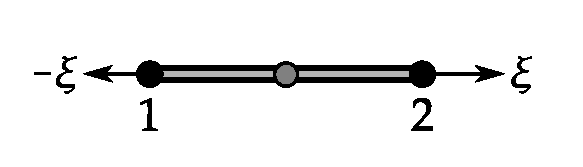
\includegraphics[width=0.3\textwidth]{figures/elements/segment_2}
  \label{fig:elements:segment2}
} & &
\subfloat[\code{\_segment\_3}]{
  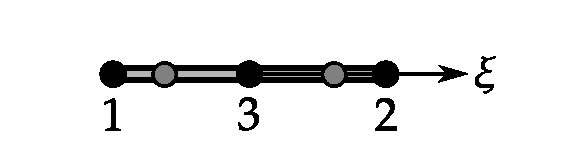
\includegraphics[width=0.3\textwidth]{figures/elements/segment_3}
  \label{fig:elements:segment3}
}
\end{tabular}
\end{center}
\caption{Schematic overview of the two 1D element types in \akantu. In each element the node numbering as used in \akantu is indicated and also the quadrature points are highlighted (gray circles).}
\label{fig:elements:1D}
\end{figure}

\begin{table}[!htb]
\begin{center}
\begin{tabular}{l|ccc}
\toprule
Element type & Order & \# nodes & \# quad. points \\
\midrule
\texttt{\_segment\_2} & linear & 2 & 1 \\
\texttt{\_segment\_3} & quadratic & 3 & 2 \\
\bottomrule
\end{tabular}
\end{center}
\caption{Some basic properties of the two 1D isoparametric elements in \akantu.}
\label{tab:elements:1D}
\end{table}

%%%%%%%%%% 2D %%%%%%%%%
\subsection*{2D\index{Elements!2D}}

In \akantu there are four types of isoparametric elements defined in 2D. These element types are called \code{\_triangle\_3}, \code{\_triangle\_6}, \code{\_quadrangle\_4} and \code{\_quadrangle\_8} and all of them are depicted in Figure~\ref{fig:elements:2D}. As with the 1D elements, some of the most basic properties of these elements are listed in Table~\ref{tab:elements:2D}. It is important to note that the first element is linear, the next two quadratic and the last one cubic. Furthermore, the last element type (\code{\_quadrangle\_8}) is not a Langrangian but a serendipity element.

\begin{figure}[!htb]
\begin{center}
\begin{tabular}{m{0.3\textwidth}m{0.1\textwidth}m{0.3\textwidth}}
\subfloat[\code{\_triangle\_3}]{
  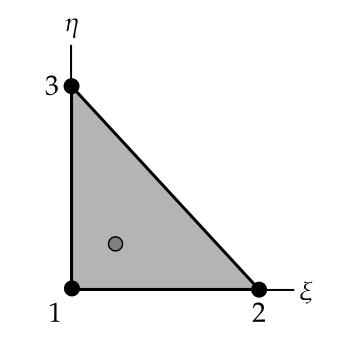
\includegraphics[width=0.3\textwidth]{figures/elements/triangle_3}
  \label{fig:elements:triangle3}
} & &
\subfloat[\code{\_triangle\_6}]{
  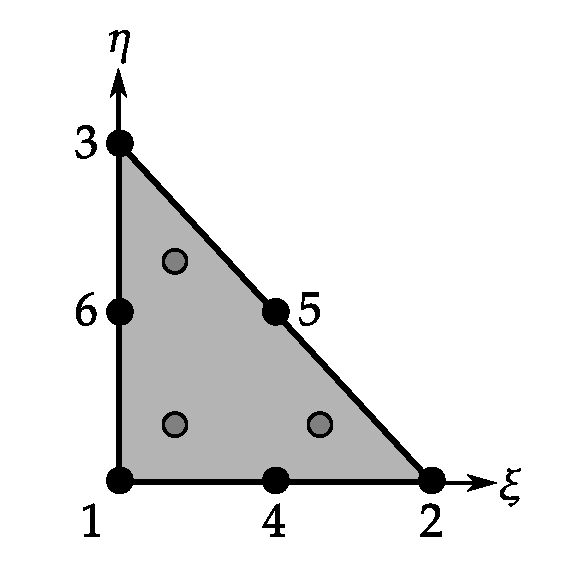
\includegraphics[width=0.3\textwidth]{figures/elements/triangle_6}
  \label{fig:elements:triangle6}
} \\
\subfloat[\code{\_quadrangle\_4}]{
  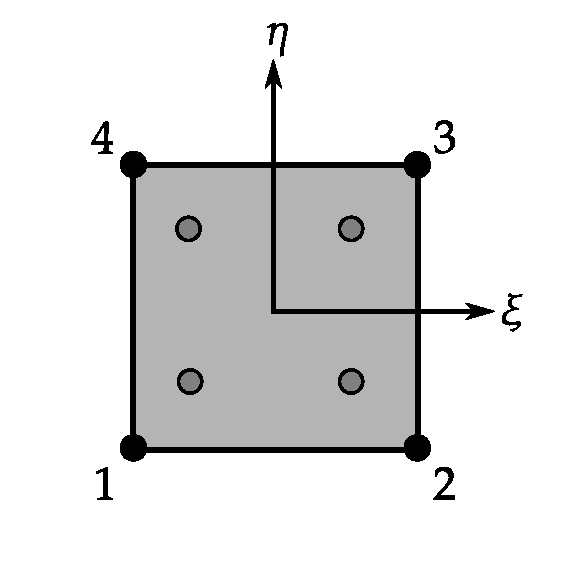
\includegraphics[width=0.3\textwidth]{figures/elements/quadrangle_4}
  \label{fig:elements:quadrangle4}
} & &
\subfloat[\code{\_quadrangle\_8}]{
  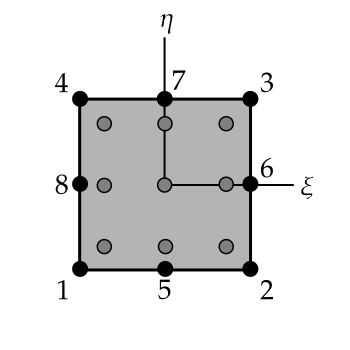
\includegraphics[width=0.3\textwidth]{figures/elements/quadrangle_8}
  \label{fig:elements:quadrangle8}
}
\end{tabular}
\end{center}
\caption{Schematic overview of the four 2D element types in \akantu. In each element the node numbering as used in \akantu is indicated and also the quadrature points are highlighted (gray circles).}
\label{fig:elements:2D}
\end{figure}

\begin{table}[!htb]
\begin{center}
\begin{tabular}{l|ccc}
\toprule
Element type & Order & \# nodes & \# quad. points \\
\midrule
\texttt{\_triangle\_3} & linear & 3 & 1 \\
\texttt{\_triangle\_6} & quadratic & 6 & 3 \\
\hline
\texttt{\_quadrangle\_4} & quadratic & 4 & 4 \\
\texttt{\_quadrangle\_8} & cubic & 8 & 9 \\
\bottomrule
\end{tabular}
\end{center}
\caption{Some basic properties of the four 2D isoparametric elements in \akantu.}
\label{tab:elements:2D}
\end{table}

%%%%%%%%%% 3D %%%%%%%%%
\subsection*{3D\index{Elements!3D}}

In \akantu there are three types of isoparametric elements defined in 3D. These element types are called \code{\_tetrahedron\_4}, \code{\_tetrahedron\_10} and \code{\_hexahedron\_8} and all of them are depicted schematically in Figure~\ref{fig:elements:3D}. As with the 1D and 2D elements some of the most basic properties of these elements are listed in Table~\ref{tab:elements:3D}.

\begin{figure}[!htb]
\begin{center}
\begin{tabular}{m{0.3\textwidth}m{0.3\textwidth}m{0.3\textwidth}}
\subfloat[\code{\_tetrahedron\_4}]{
  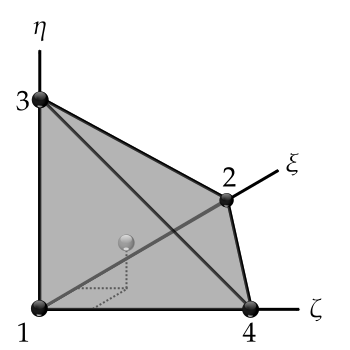
\includegraphics[width=0.3\textwidth]{figures/elements/tetrahedron_4}
  \label{fig:elements:tetrahedron4}
} &
\subfloat[\code{\_tetrahedron\_10}]{
  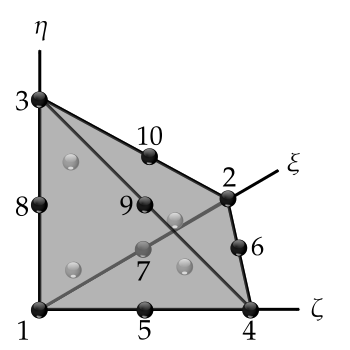
\includegraphics[width=0.3\textwidth]{figures/elements/tetrahedron_10}
  \label{fig:elements:tetrahedron10}
} &
\subfloat[\code{\_hexahedron\_8}]{
  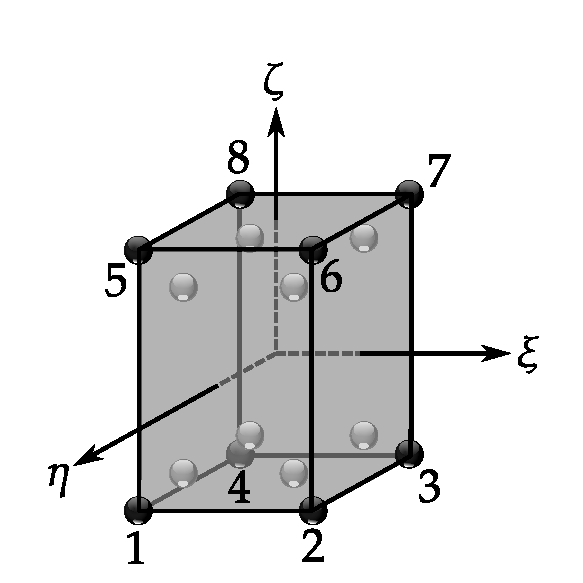
\includegraphics[width=0.3\textwidth]{figures/elements/hexahedron_8}
  \label{fig:elements:hexahedron8}
}
\end{tabular}
\caption{Schematic overview of the three 3D element types in \akantu. In each element the node numbering as used in \akantu is indicated and also the quadrature points are highlighted (gray spheres).}
\label{fig:elements:3D}
\end{center}
\end{figure}

\begin{table}[!htb]
\begin{center}
\begin{tabular}{l|ccc}
\toprule
Element type & Order & \# nodes & \# quad. points  \\
\midrule
\texttt{\_tetrahedron\_4} & linear & 4 & 1  \\
\texttt{\_tetrahedron\_10} & quadratic & 10 & 4  \\
\hline
\texttt{\_hexahedron\_8} & cubic & 8 & 8  \\
\bottomrule
\end{tabular}
\end{center}
\caption{Some basic properties of the three 3D isoparametric elements in \akantu.}
\label{tab:elements:3D}
\end{table}


%%%%%%%%%% COHESIVE ELEMENTS %%%%%%%%%
\IfFileExists{manual-cohesive_elements.tex}{
\section{Cohesive elements}

Cohesive elements are a numerical tool that lets a crack propagate
along the edges of standard elements. The cohesive elements that have
been implemented in Akantu are based on the work of Ortiz and
Pandolfi~\cite{ortiz1999}.

\begin{figure}
  \centering
  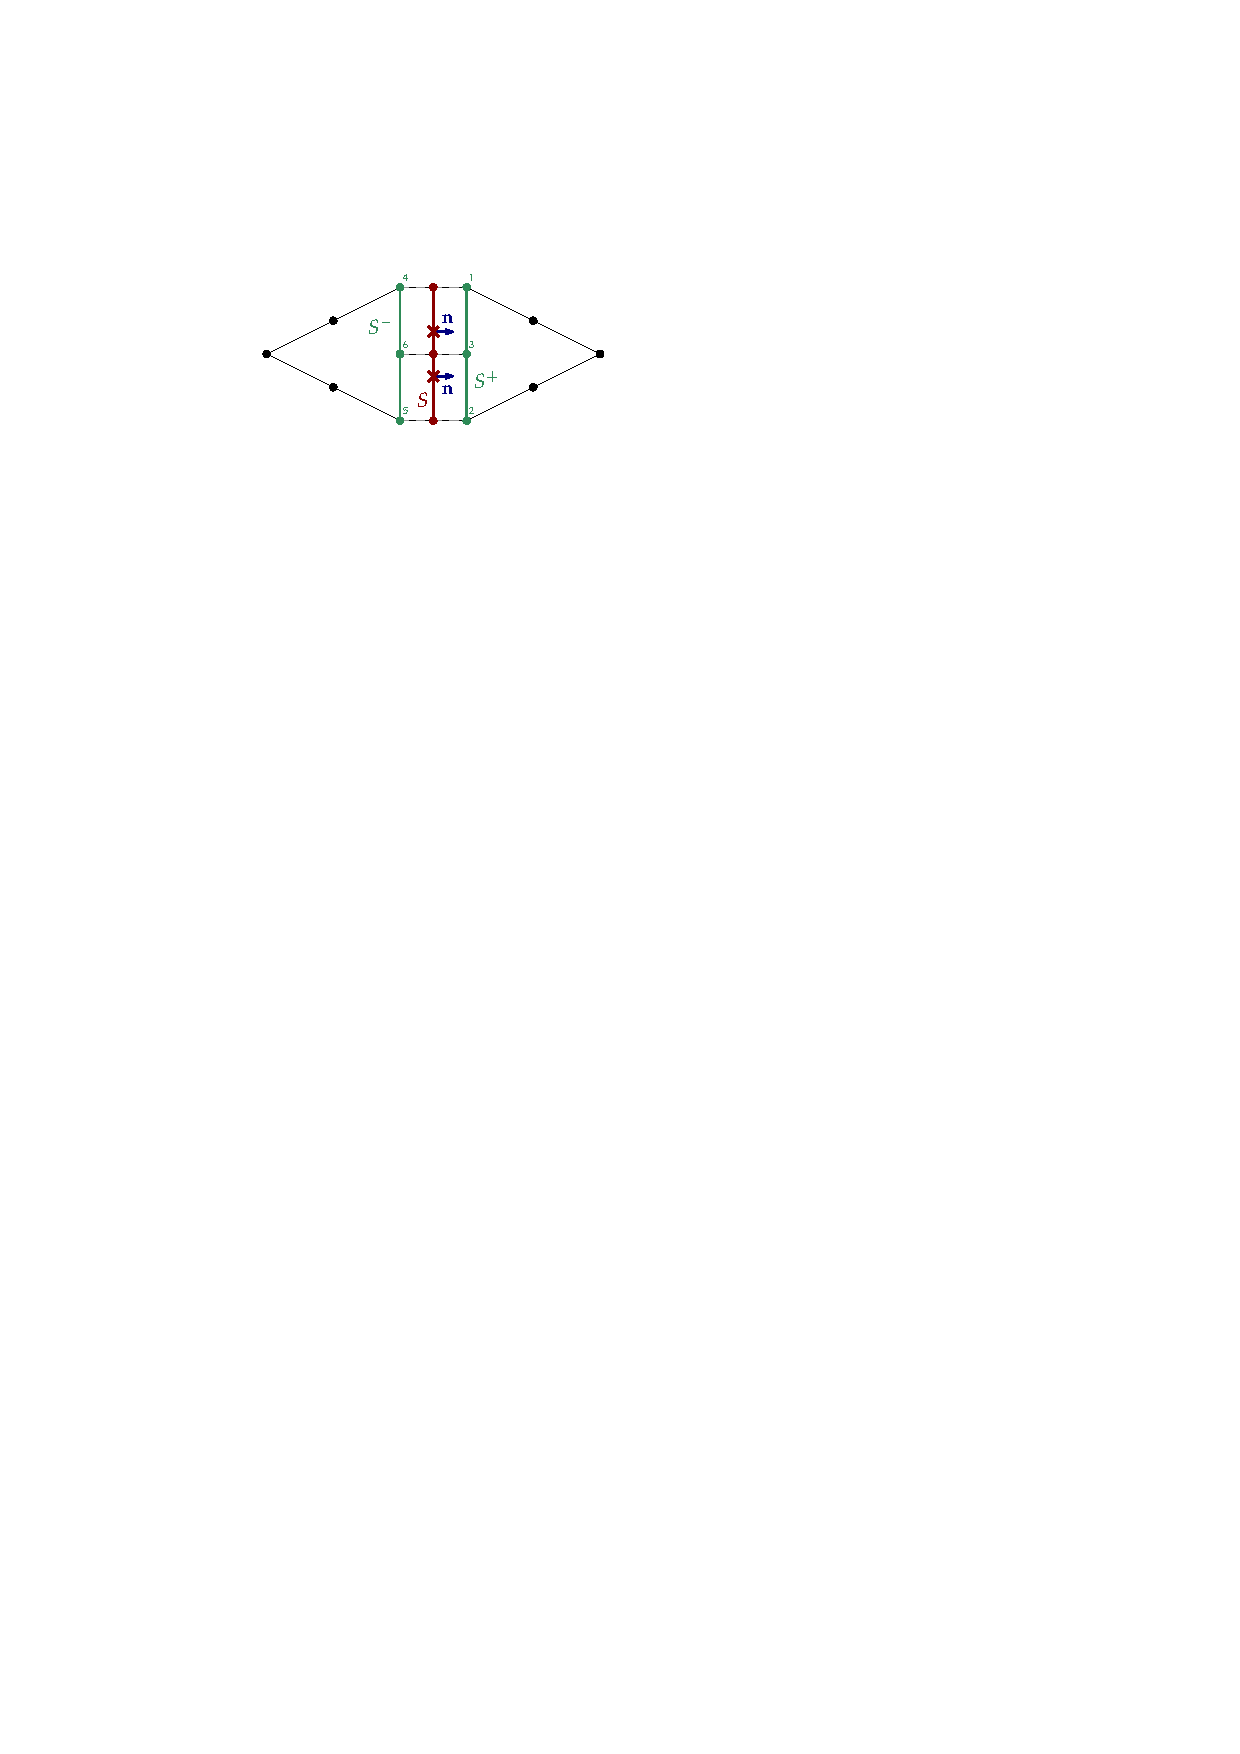
\includegraphics[width=.6\textwidth]{figures/cohesive2d}
  \caption{Cohesive element in 2D for quadratic triangular elements
    T6.}
  \label{fig:smm:coh:cohesive2d}
\end{figure}

\begin{figure}
  \centering
  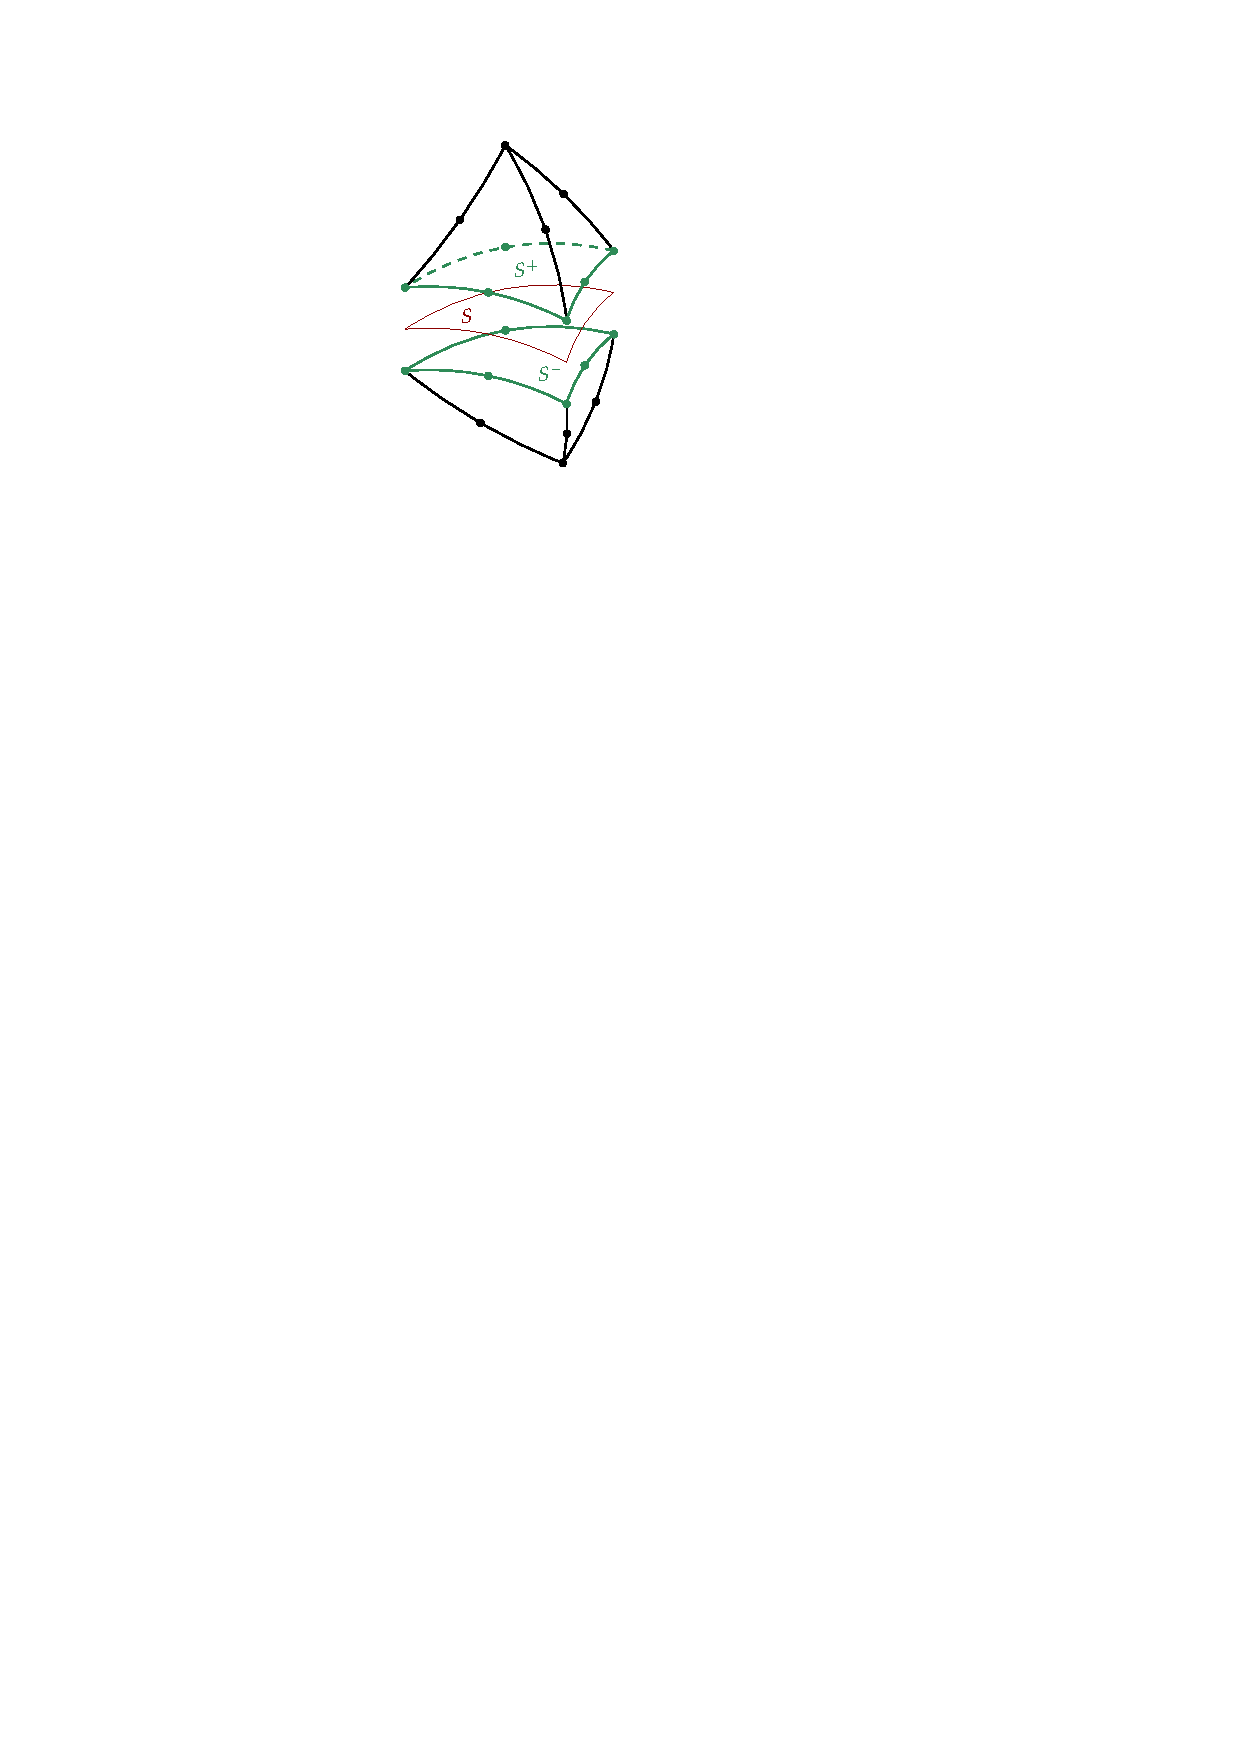
\includegraphics[width=.25\textwidth]{figures/cohesive3d}
  \caption{Cohesive element in 3D for quadratic tetrahedrons T10.}
  \label{fig:smm:coh:cohesive3d}
\end{figure}

Cohesive elements consist of a couple of surface elements which are
coincident in space when the opening displacement is zero. Two
schematics of cohesive elements in 2D and 3D can be seen in
figures~\ref{fig:smm:coh:cohesive2d}
and~\ref{fig:smm:coh:cohesive3d}. The two surface elements, denoted by
$S^-$ and $S^+$, must be of the same type and they correspond to the
facet element of the standard elements. All the computations are done
on the middle surface $S$, whose nodal coordinates are just the
average between those of $S^+$ and $S^-$.

In order to track normal and tangential openings, it is convenient to
define a unique normal direction $\vec{n}$ for each quadrature point
of the cohesive element. By convention the normal points from $S^-$ to
$S^+$. The opening displacement vector is:
\begin{equation}
  \label{eq:opening_displacement}
  \vec{\Delta} (\vec{s}) = \sum_{n=1}^N \llbracket \vec{x}_n \rrbracket N_n (\vec s)
\end{equation}
where $N_n$ are the shape functions of the cohesive element (they are
exactly the same of those of a single surface element) and
\begin{equation}
  \label{eq:disp_difference}
  \llbracket \vec{x}_n \rrbracket = \vec{x}_n^+ - \vec{x}_n^-
\end{equation}
in which $\vec{x}_n^\pm$ for $n=1,\dots,N$ are the current coordinates
of the nodes.

The quantities that have been defined so far are sufficient to
completely define the cohesive tractions per unit deformed
area. As the tangential direction $\vec{t}$ depends on the normal one
$\vec{n}$, equation~\eqref{eq:smm:coh:tractions} can be rewritten as:
\begin{equation}
  \vec{T} = \left[ \frac{\beta^2}{\kappa} \vec{\Delta} +
    \left( 1- \frac{\beta^2}{\kappa}\right)
    \left( \vec{\Delta} \cdot \vec{n}\right) \vec{n} \right]
  \frac{\sigma_\mathrm{c}}{\delta}
  \left( 1- \frac{\delta}{\delta_\mathrm{c}} \right) =
  \vec{T}(\vec{\Delta}, \vec{n})
\end{equation}
 By interpolation it is now possible to derive the nodal
forces as:
\begin{equation}
  f_{in}^\pm = \mp \int_{S_0} T_i N_n\, \mathrm{d}S_0
\end{equation}
in which the integral extends over the undeformed middle surface $S_0$
of the cohesive element.

\begin{figure}
  \centering
  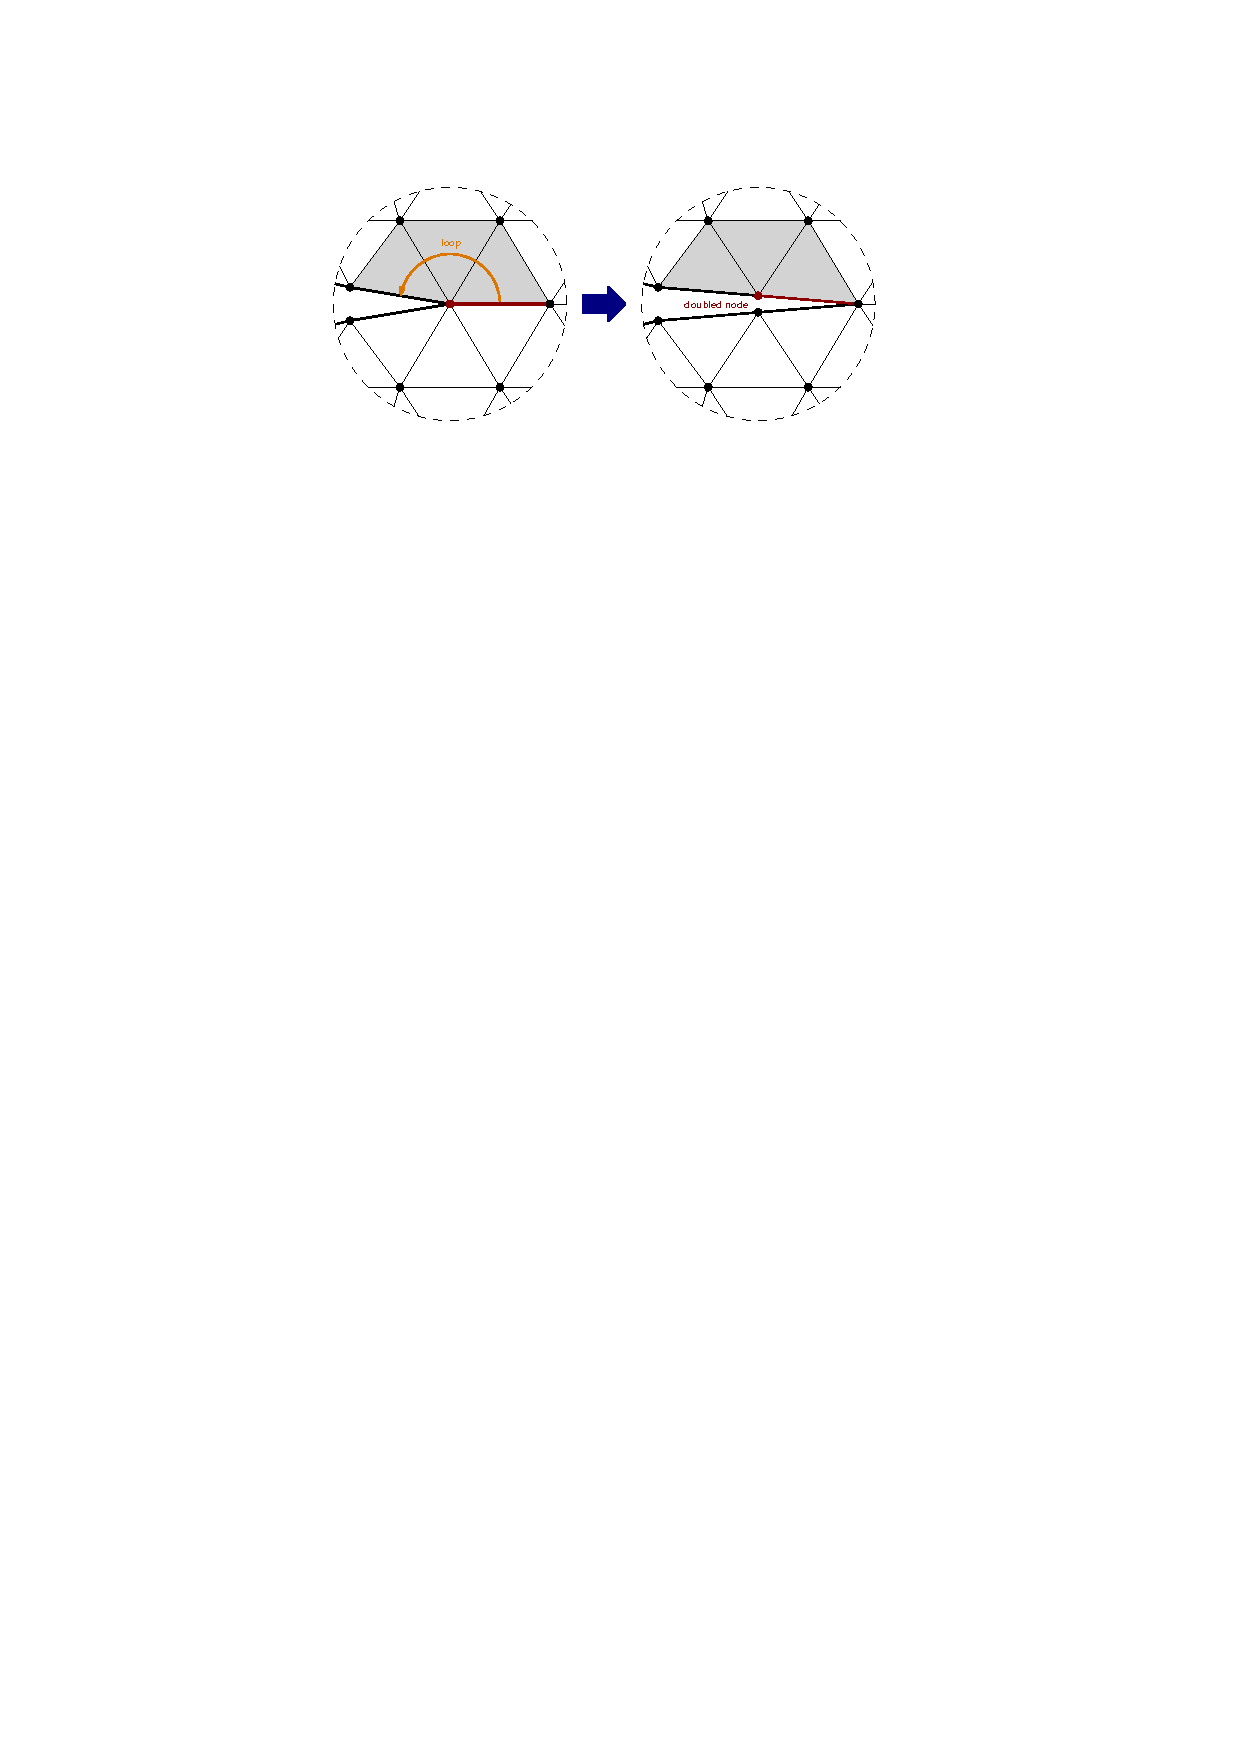
\includegraphics[width=.9\textwidth]{figures/insertion}
  \caption{Insertion of a cohesive element.}
  \label{fig:smm:coh:insertion}
\end{figure}

Cohesive element insertion can be either realized at the beginning of
the simulation or it can be carried out dynamically during the
simulation. The first approach is called \emph{intrinsic} while the
second one \emph{extrinsic}. When an element is present from the
beginning, a bilinear or exponential cohesive law should be used
instead of a linear one. A bilinear law works exactly like a linear
one except for an additional parameter $\delta_0$ separating an
initial linear elastic part from the linear irreversible one. The
exponential law will be described later in the manual.

In dynamic cohesive element insertion, normal and tangential stresses
along the edges of standard elements are used to compute the effective
stress
\begin{equation}
  \sigma_\mathrm{eff} = \sqrt{\sigma_\mathrm{n}^2 +
    \frac{\tau_\mathrm{nt}^2}{\beta^2}}
\end{equation}
where the indexes $n$ and $t$ respectively refer to normal and
tangential directions. Obviously, if $\sigma_\mathrm{n}$ is
compressive, its contribution is not considered. The so computed
effective stress $\sigma_\mathrm{eff}$ is monitored, and when it
overcomes a threshold stress on a certain edge a new cohesive element
is inserted. New nodes are added and the element connectivity is
updated (see figure~\ref{fig:smm:coh:insertion}). This topological
mesh changing technique is very convenient because it allows
simulating crack propagation without remeshing the domain.

\begin{table}[!htb]
\begin{center}
\begin{tabular}{l|llcc}
\toprule
Element type & Facet type & Order & \# nodes & \# quad. points  \\
\midrule
\texttt{\_cohesive\_1d\_2} & \texttt{\_point\_1} & linear & 2 & 1  \\
\hline
\texttt{\_cohesive\_2d\_4} & \texttt{\_segment\_2} & linear & 4 & 1  \\
\texttt{\_cohesive\_2d\_6} & \texttt{\_segment\_3} & quadratic & 6 & 2  \\
\hline
\texttt{\_cohesive\_3d\_6} & \texttt{\_triangle\_3} & linear & 6 & 1  \\
\texttt{\_cohesive\_3d\_12} & \texttt{\_triangle\_6} & quadratic & 12 & 3  \\
\bottomrule
\end{tabular}
\end{center}
\caption{Some basic properties of the cohesive elements in \akantu.}
\label{tab:cohesive_elements}
\end{table}

%%% Local Variables:
%%% mode: latex
%%% TeX-master: "manual"
%%% End:
}{}

%%%%%%%%%% STRUCTURAL ELEMENTS %%%%%%%%%
\IfFileExists{manual-structuralmechanicsmodel-elements.tex}{\subsection{Structural Elements\index{Elements!Structural}}

\subsubsection*{Bernoulli Beam Elements\index{Elements!Bernoulli}}
These elements allow to compute the displacements and rotations of
structures constituted by Bernoulli beams. \akantu defines them for
both 2D and 3D problems respectively in the element types
\code{\_bernoulli\_beam\_2} and \code{\_bernoulli\_beam\_3}. A
schematic depiction of a beam element is shown in
Figure~\ref{fig:elements:bernoulli} and some of its properties are
listed in Table~\ref{tab:elements:bernoulli}.

\note{Beam elements are of mixed order: the axial displacement is
  linearly interpolated while transverse displacements and rotations
  use cubic shape functions.}

\begin{figure}[htb]
  \centering
  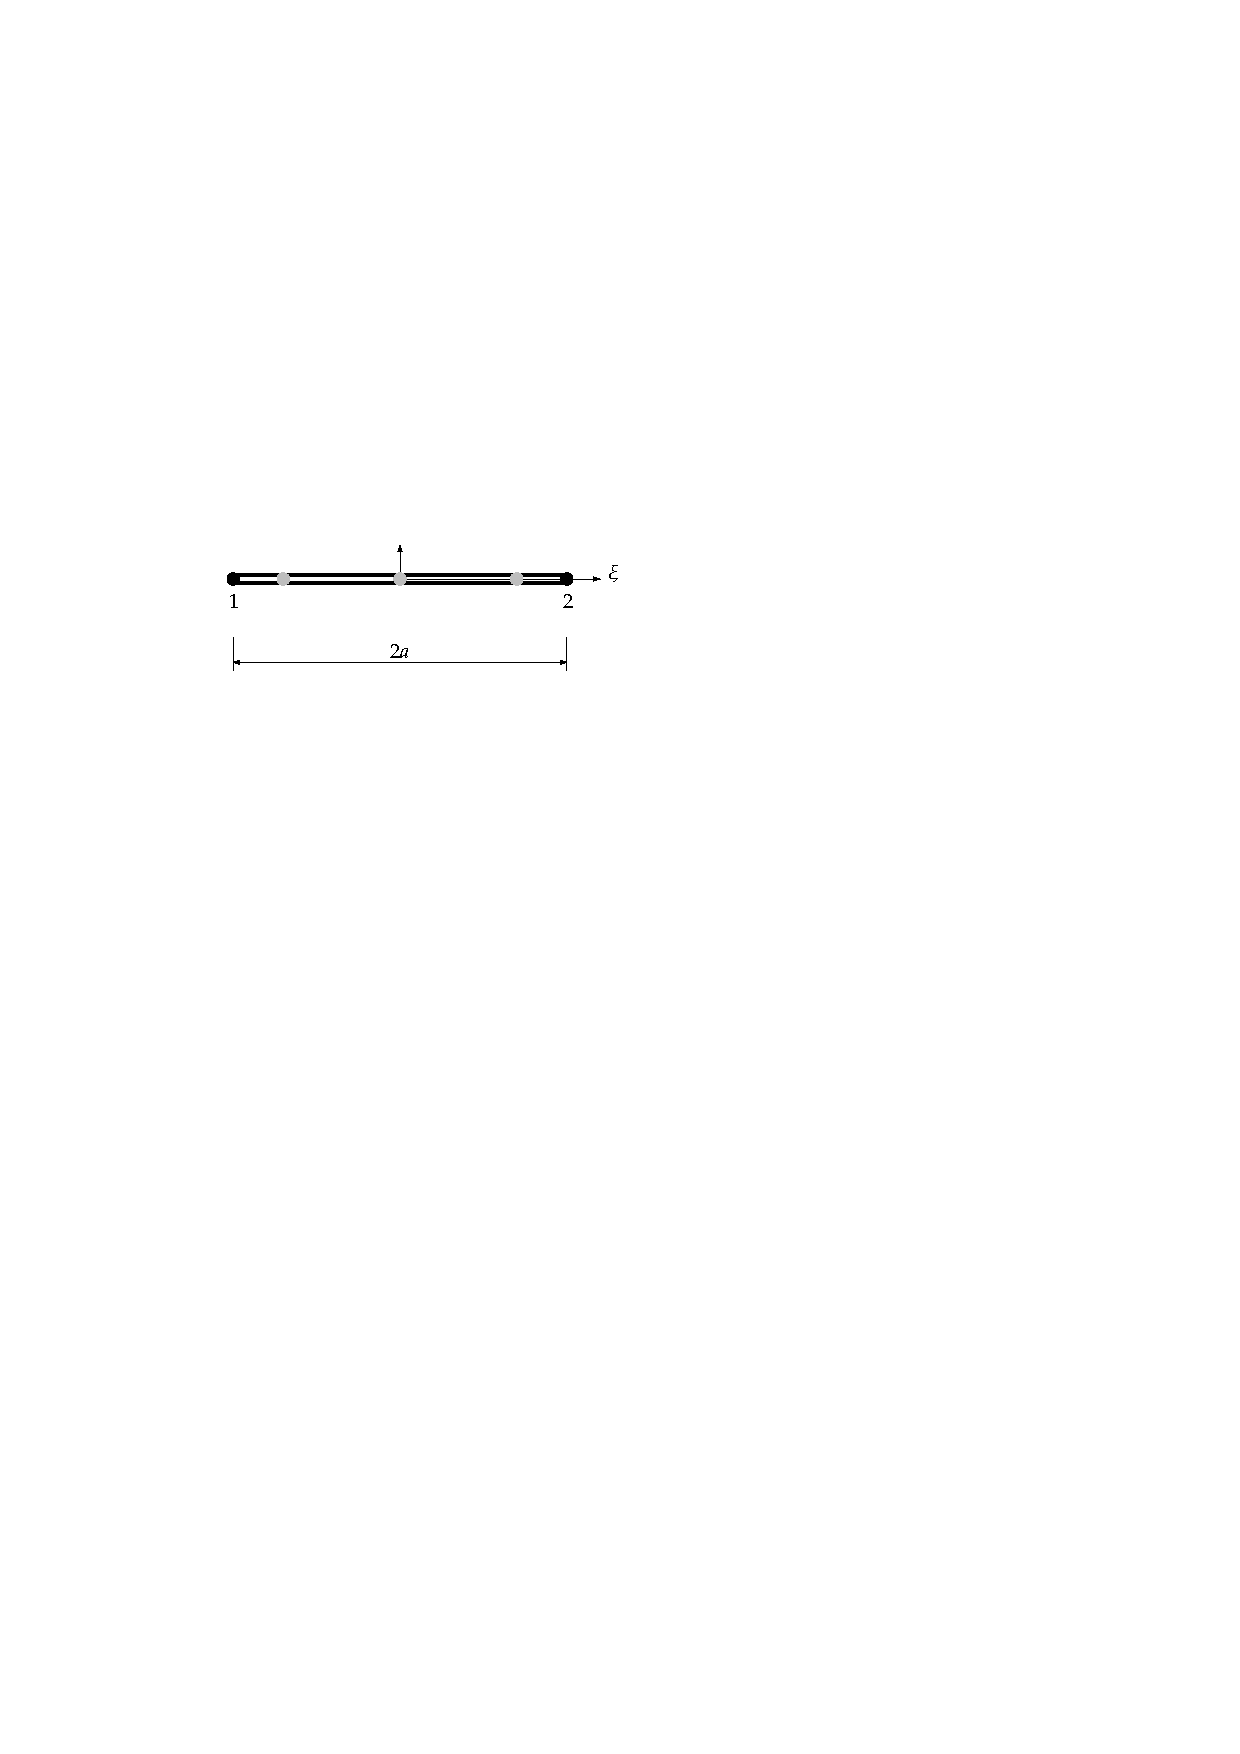
\includegraphics[width=0.3\textwidth]{figures/elements/bernoulli_2}
  \caption{Schematic depiction of a Bernoulli beam element (applied to
    2D and 3D) in \akantu. The node numbering as used in \akantu is
    indicated, and also the quadrature points are highlighted (gray
    circles).}
  \label{fig:elements:bernoulli}
\end{figure}
\begin{table}[htb]
  \centering
  \begin{tabular}{c|cccc}
    \toprule
    Element type                  & Dimension & \# nodes &\# quad. points & \# d.o.f.\\
    \midrule
    \texttt{\_bernoulli\_beam\_2} &         2D&         2&              3&  6\\
    \texttt{\_bernoulli\_beam\_3} &         3D&         2&              3&  12\\
    \bottomrule
  \end{tabular}
  \caption{Some basic properties of the beam elements in \akantu}
  \label{tab:elements:bernoulli}
\end{table}
}{}

%%% Local Variables:
%%% mode: latex
%%% TeX-master: "manual"
%%% End:

